\documentclass{article}

\usepackage{amsmath, amssymb}
\usepackage{float}
\usepackage{graphicx}
\usepackage{subcaption}
\usepackage{color}

\usepackage{listings}


\definecolor{dkgreen}{rgb}{0,0.6,0}
\definecolor{gray}{rgb}{0.5,0.5,0.5}
\definecolor{mauve}{rgb}{0.58,0,0.82}

\lstset{frame=tb,
  language=python,
  aboveskip=3mm,
  belowskip=3mm,
  showstringspaces=false,
  columns=flexible,
  basicstyle={\small\ttfamily},
  numberstyle=\color{gray},
  keywordstyle=\color{blue},
  commentstyle=\color{dkgreen},
  stringstyle=\color{mauve},
  breaklines=true,
  breakatwhitespace=true,
  tabsize=3,
}
%

\addtolength{\topmargin}{-.875in}
\addtolength{\textheight}{1.75in}


\title{Project report - Week 1}
\date{May 10, 2020}

\begin{document}
	\maketitle
\section{Introductory information}
	\subsection{Dataset}
		The dataset used for this project consist of 17 types of flowers, each one represented by 80 images. 
		The images were split in 70/10 ratio for training and validation.
	\subsection{Neural Network}
		 For the problem of image recognition the convolutional neural network was chosen.
		 It was built using 3 convolutional and 3 max pooling layers,  with two densely-connected layers on top.
\section{Training results}
	\subsection{Number of epochs}
		\begin{figure}[h!]
			\centering
			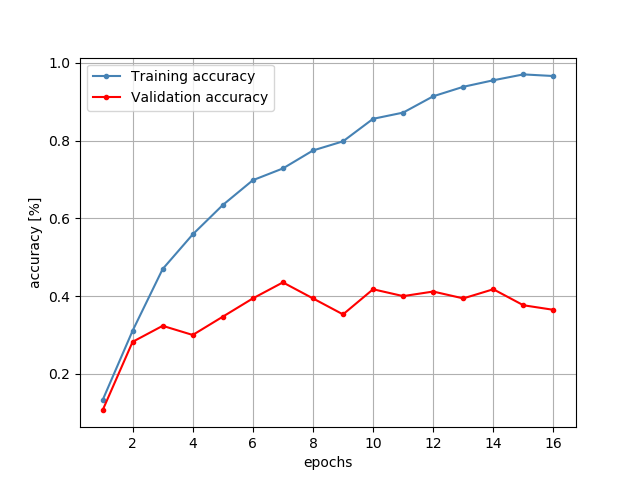
\includegraphics[width = \textwidth]{img/epochs}
			\caption{Results of training network for 16 epochs. Images were scaled to 64x64 pixel size.}
			\label{fig:epochs}		
		\end{figure}
		As seen on fig.\ref{fig:epochs} the network is prone to overfitting. It is probably effect of fairly small number of images in the dataset.
		After about 8 epochs accuracy of network over validation dataset doesn't improve anymore.
	\subsection{Image size}
		\begin{figure}[h!]
			\centering
			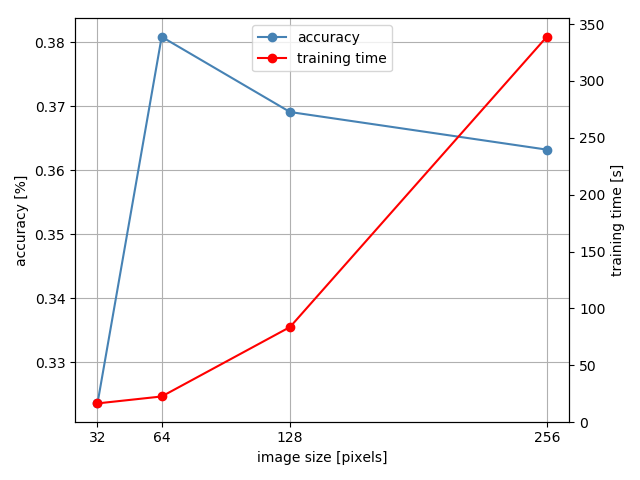
\includegraphics[width = \textwidth]{img/sizes}
			\caption{Time required to train network for 8 epochs with images of given size and achieved accuracy.}					
		\end{figure}
		Increasing size of the input image doesn't seem to improve model's accuracy, but greatly increases time required for training.
		Because of this, image size chosen for the network input was 64x64 pixels.
\section{Summary}
	While training network with parameters from section 2 (i.e. 8 epochs and image size of 64x64 pixels), achieved accuracy oscillated around 40\%.
	Biggest obstacle for getting better accuracy is at the moment strong overfitting of the network.
\end{document}